%%! TEX program=xelatex

\documentclass{article}
\usepackage{mathtools}
\usepackage{graphicx}
\usepackage{verbatim}
\usepackage{tikz}
\usepackage{pgfplotstable}
\usepackage{pgfplots}
\usepackage{bm}
\usepackage[colorlinks,urlcolor=blue,citecolor=red,linkcolor=red]{hyperref}

\title{TinyTeX-mmCEsim Test}
\author{Wuqiong Zhao}
\date{\today}

\listfiles
\begin{document}

  \maketitle

  \section{Brief}
    This is a test of \href{https://github.com/mmcesim/tinytex-mmcesim}{TinyTeX-mmCEsim}.

  \section{Graphics}
    
    Example image is shown in Fig.~\ref{fig:example}.
    \begin{figure}[htbp]
      \centering
      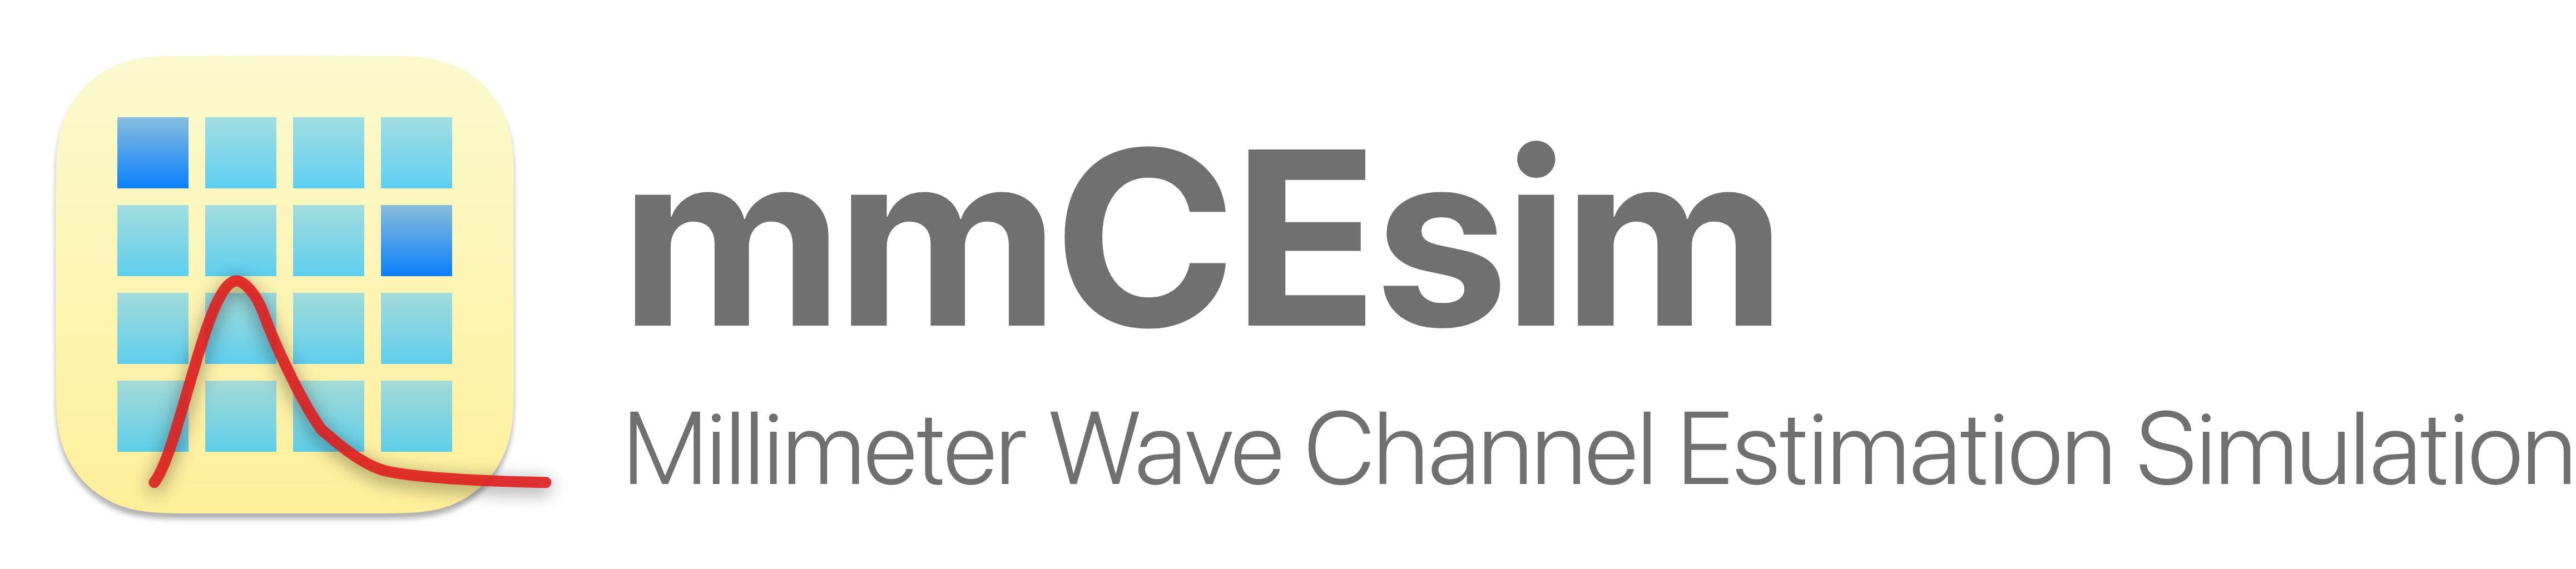
\includegraphics[width=\linewidth]{mmCEsim_badge.png}
      \caption{mmCEsim badge.}
      \label{fig:example}
    \end{figure}

  \section{Maths}

    One equation
    \begin{equation}
      \mathbf{y}_k=\mathbf{H}_k\mathbf{x}_k+\mathbf{n},
    \end{equation}
    and another one
    \begin{equation}
      y=|x|=
      \left\{
        \begin{aligned}
          x&,\quad x\geq0\\
          -x&,\quad\mathrm{otherwise}.
        \end{aligned}
      \right.
    \end{equation}
    
    Let's test \verb+\bm{}+ command: $\bm{\Psi}$.

  \newpage
  \section{TikZ}

    \begin{figure}[htbp]
      \centering
      \begin{tikzpicture}
        \begin{axis}[
          xlabel=Q Series,
          ylabel=P Values]
          \addplot table [y=P, x=$Q_A$]{data.dat};
          \addlegendentry{$Q_A$ series}
          \addplot table [y=P, x=$Q_B$]{data.dat};
          \addlegendentry{$Q_B$ series}
          \addplot table [y=P, x=$Q_D$]{data.dat};
          \addlegendentry{$Q_D$ series}
        \end{axis}
      \end{tikzpicture}
      \caption{Ti\textit{k}Z test.}
    \end{figure}
  
\end{document}
